\section*{Meta Activity: POGIL Research 2}

Many research studies have been conducted about POGIL.
In the following example, students were given an unannounced quiz on the first day of class (based on the previous semester).
About half of them had been taught in lecture sections, and half in POGIL sections.

\begin{center}
% image from Chapter 8 of http://dx.doi.org/10.7936/K7PN93HC
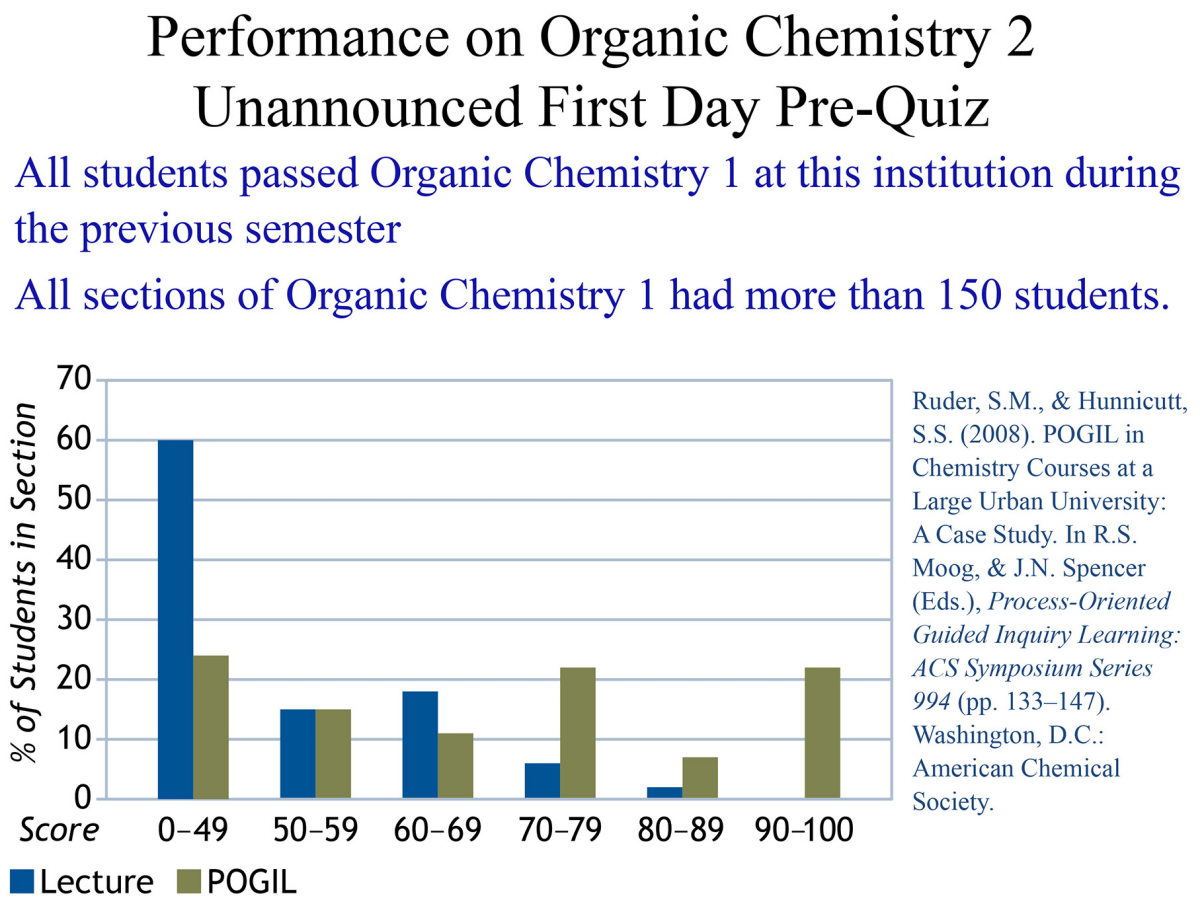
\includegraphics[width=0.625\linewidth]{pogil-prequiz.png}
\end{center}


\quest{7.5 min}


\Q How large were the classes in the previous semester?

\begin{answer}[2em]
More than 150 students per section.
\end{answer}

\vspace{1ex}


\Q About what percentage of the \ldots

\begin{multicols}{2}
\begin{enumerate}

\item Lecture students scored below 60? \ans[2em]{75}
%\item Lecture students scored above 60? \ans[2em]{25}
\item Lecture students scored above 80? \ans[2em]{2}

\item POGIL students scored below 60? \ans[2em]{38}
%\item POGIL students scored above 60? \ans[2em]{62}
\item POGIL students scored above 80? \ans[2em]{30}

\end{enumerate}
\end{multicols}


\Q What does the research suggest about students' retention of knowledge?

\begin{answer}[5em]
Students in courses that use POGIL are more likely to remember what they learn:
``In contrast, fewer than a quarter of the students from the POGIL section scored below 50 percent on this quiz, and about 30 percent of the students scored above 80 percent, with over one-fifth of the POGIL students scoring above 90 percent.'' (Moog 2014)
\end{answer}
